\documentclass[hidelinks,11pt,dvipsnames]{article}
% xcolor commonly causes option clashes, this fixes that
\PassOptionsToPackage{dvipsnames,table}{xcolor}
\usepackage[tmargin=1in, bmargin=1in, lmargin=0.8in, rmargin=1in]{geometry}

%%%%%%%%%%%%%%%%%%%%%%%%%%%%%%%%%%%%%%%%%%%%%%%%%%%%%%%%%%%%%%%%%%%%
%%% For inkscape-figures
%%% Assumes the following directory structure:
%%% master.tex
%%% figures/
%%%     figure1.pdf_tex
%%%     figure1.svg
%%%     figure1.pdf
%%%%%%%%%%%%%%%%%%%%%%%%%%%%%%%%%%%%%%%%%%%%%%%%%%%%%%%%%%%%%%%%%%%%
%\usepackage{import}
\usepackage{pdfpages}
\usepackage{transparent}

\newcommand{\incfig}[2][1]{%
    \def\svgwidth{#1\columnwidth}
    \import{./figures/}{#2.pdf_tex}
}

\pdfsuppresswarningpagegroup=1

% enable synctex for inverse search, whatever synctex is
\synctex=1
\usepackage{float,macrosabound,homework,theorem-env}
\usepackage{microtype}


% font stuff
\usepackage{sectsty}
\allsectionsfont{\sffamily}
\linespread{1.1}

% bibtex stuff
\usepackage[backend=biber,style=alphabetic,sorting=anyt]{biblatex}
\addbibresource{main.bib}

% colored text shortcuts
\newcommand{\blue}[1]{\color{MidnightBlue}{#1}}
\newcommand{\red}[1]{\textcolor{Mahogany}{#1}}
\newcommand{\green}[1]{\textcolor{ForestGreen}{#1}}


% use mathptmx pkg while using default mathcal font
\DeclareMathAlphabet{\mathcal}{OMS}{cmsy}{m}{n}

% fixes the positioning of subscripts in $$ $$
\renewcommand{\det}{\operatorname{det}}

\usetikzlibrary{positioning, arrows.meta}
\newcommand{\here}[2]{\tikz[remember picture]{\node[inner sep=0](#2){#1}}}

%%%%%%%%%%%%%%%%%%%%%%%%%%%%%%%%%%%%%%%%%%%%%%%%%%%%%%%%%%%%%%%%%%%%%
%%% Entry Counter
%%%%%%%%%%%%%%%%%%%%%%%%%%%%%%%%%%%%%%%%%%%%%%%%%%%%%%%%%%%%%%%%%%%%%
\newcounter{entry-counter}
\newcommand{\entry}[1]
{
	\addtocounter{entry-counter}{1}
    \tchap{Entry \arabic{entry-counter}}
	%\addcontentsline{toc}{section}{Entry \arabic{entry-counter}: #1}
	\vspace{-1.5em}
    \begin{center}
		\small \emph{Written: #1}
    \end{center}
}

\usepackage{titling}
\renewcommand\maketitlehooka{\null\mbox{}\vfill}
\renewcommand\maketitlehookd{\vfill\null}


\usepackage{capt-of}
\usepackage{tikz}
\usetikzlibrary{positioning,calc,intersections,through,backgrounds, shapes.geometric, decorations.markings,arrows}

\def\sset{\subseteq}
\def\iso{\cong}
\def\gend#1{\langle #1\rangle}

\newcommand{\rightoverleftarrow}{%
  \mathrel{\vcenter{\mathsurround0pt
    \ialign{##\crcr
      \noalign{\nointerlineskip}$\longrightarrow$\crcr
      \noalign{\nointerlineskip}$\longleftarrow$\crcr
    }%
  }}%
}

\newcommand\makesphere{} % just for safety
\def\makesphere(#1)(#2)[#3][#4]{%
  % Synopsis
  % \makesphere[draw options](center)(initial angle:final angle:radius)
  \shade[ball color = #3, opacity = #4] #1 circle (#2);
  \draw #1 circle (#2);
  \draw ($#1 - (#2, 0)$) arc (180:360:#2 and 3*#2/10);
  \draw[dashed] ($#1 + (#2, 0)$) arc (0:180:#2 and 3*#2/10);
}
% same thing as makesphere but places white background behind
\newcommand\altmakesphere{} % just for safety
\def\altmakesphere(#1)(#2)(#3)[#4][#5]{%
  % Synopsis
  % \make sphere[draw options](center)(initial angle:final angle:radius)
  \draw [fill=white!30] #1 circle (#2);
  \shade[ball color = #4, opacity = #5] #1 circle (#2);
  \draw #1 circle (#2);
  \draw ($#1 - (#2, 0)$) arc (180:360:#2 and 3*#2/10);
  \draw[dashed] ($#1 + (#2, 0)$) arc (0:180:#2 and 3*#2/10);
  \node at #1 {#3};
}

\begin{document}
% set section number to 1
% fixes theorem numbering without need to have a section title
\setcounter{section}{1}

\pagestyle{empty}
	\LARGE
\begin{center}
	Algebraic Topology Homework 9 \\
	\Large
	Isaac Martin \\
    Last compiled \today
\end{center}
\normalsize
\vspace{-4mm}
\hru

\tchap{Problems from 2.1}

\begin{homework}[e]
  \prob[\textsc{Exercise 22.}] Prove by induction on dimension the following facts about the homology of finite-dimensional CW complex $X$, using the observation that $X^n/X^{n-1}$ is a wedge sum of $n$-spheres:
  \begin{enumerate}[(a)]
    \item If $X$ has dimension $n$ then $H_i(X) = 0$ for $i > n$ and $H_n(X)$ is free.
    \item $H_n(X)$ is free with basis in bijective correspondence with the $n$-cells if there are no cells of dimension $n-1$ or $n+1$
    \item If $X$ has $k$ $n$-cells, then $H_n(X)$ is generated by at most $k$-elements.
  \end{enumerate}
  \begin{prf}
    \noindent \textbf{(a)}\hspace{1em} First notice that we have the following series of isomorphisms:
    \begin{align*}
      H_i(X^k,X^{k-1}) \cong H_i(X^k/X^{k-1}) \cong H_i\left(\bigvee_\alpha S^k\right) \cong \bigoplus H_i(S^k) =
      \begin{cases}
        \bigoplus_\alpha \bZ & i = k \\
        0 & \text{else}
      \end{cases}
    \end{align*}
    where $i$ and $k$ are nonnegative integers and $\alpha$ indexes the $k$-cells of $X$. The first isomorphism is given by Proposition 2.22 (a special case of Theorem 2.13 when (X,A) is a good pair), the second isomorphism follows from the homeomorphism $X^k/X^{k-1}\cong \bigvee_\alpha S^k$ and the third is implied by Corollary 2.25. Now consider the following exact sequence
    \begin{align*}
      ... \to H_i(X^{n-1}) \to H_i(X^n) \to H_i(X^n,X^{n-1}) \to ...
    \end{align*}
    induced by the inclusion $X^{n-1}\hookrightarrow X^n$. Since $X$ is dimension $n$, $X = X^n$, and by the above isomorphisms, $H_i(X^n,X^{n-1})\cong 0$ when $i > n$. We therefore appeal to induction: if $H^{n-1} = 0$, then by the exactness of the above sequence, we have $H_i(X^n)\cong H_i(X^n-1) \cong 0$. For the base case, suppose $X$ were a $0$-dimensional CW-complex. Then $X$ would be a disjoint union of points, and from previous results $H_i(X) = 0$ for all $i > 0$. This proves the first portion of part (a).

    For the second part, we return to the exact sequence given by the inclusion $X^{n-1}\hookrightarrow X^n$. When $i = n$, we get that $H_n(X^{n-1}) = 0$ and so
    \begin{align*}
      ... \to 0 \to H_n(X) \to \bigoplus_\alpha \bZ \to ... 
    \end{align*}
    is the relevant portion of the sequence. By exactness, the map $H_n(X) \to \bigoplus_\alpha \bZ$ must be injective, so $H_n(X)$ is isomorphic as an abelian group to its image in $\bigoplus_\alpha \bZ$. Since all subgroups of a free abelian group are themselves free abelian, $H_n(X)$ is free abelian.
    
    \bigskip

    \noindent \textbf{(b)}\hspace{1em} Now let $n$ be some fixed integer, not necessarily the dimension of $X$, and suppose $X$ has no $(n-1)$-cells nor any $(n+1)$-cells. This means that the $(n-1)$-skeleton is equal to the $(n-2)$-skeleton, i.e. $X^{n-1} = X^{n-2}$ By part (a), it must then be the case that $H_{n}(X^{n-1}) \cong H_{n-1}(X^{n-1}) \cong 0$, and so the exact sequence
    \begin{align*}
      ... \to H_n(X^{n-1}) \to H_n(X) \to H_n(X^n,X^{n-1}) \to H_{n-1}(X^{n-1}) \to ...
    \end{align*}
    can actually be written
    \begin{align*}
      ... \to 0 \to H_n(X) \to H_n(X^n,X^{n-1}) \to 0 \to ...
    \end{align*}
    which implies that $H_n(X) \cong H_n(X,X^{n-1})$ by exactness.

    As we saw in part (a), $H_n(X^n,X^{n-1})$ is the free group generated by $n$-cells, so if we can show $H_n(X,X^{n-1}) \cong H_n(X^n,X^{n-1})$ we'll be done. For this, we'll make use of the short exact sequence 
    \begin{align*}
      0 \to C_n(X^n,X^{n-1}) \to C_n(X,X^{n-1}) \to C_n(X,X^n) \to 0
    \end{align*}
    to obtain the following long exact sequence on homology:
    \begin{align*}
      ... \to H_{n+1}(X,X^n) \to H_n(X^n,X^{n-1}) \to H_n(X,X^{n-1}) \to H_n(X,X^{n}) \to ...
    \end{align*}
    By part (a), we know that $H_i(X^n,X^{n-1}) = 0$ whenever $i \neq n$. Furthermore, because there are no $(n+1)$-cells, $X^{n+1} = X^n$ and hence $H_{n+1}(X,X^n) = 0$. To see that $H_n(X,X^n) \cong 0$, consider the long exact sequence of the pair $(X,X^n)$:
    \begin{align*}
      ... \to H_n(X^n) \xrightarrow{\alpha} H_n(X) \to H_n(X)\to H_n(X,X^n) \to H_{n-1}(X_n) \xrightarrow{\beta} H_{n-1}(X) \to ...
    \end{align*}
    I claim that $\alpha$ is injective, $\beta$ is surjective and hence by problem 2.1.15 $H_n(X,X^n) \cong 0$. Indeed, the exactness of
    \begin{align*}
      ... \to H_{i+1}(X^n,X^{n-1}) \to H_i(X^{n-1}) \xrightarrow{\alpha} H_i(X^{n}) \xrightarrow{\beta} H_i(X^n,X^{n-1}) \to ...
    \end{align*}
    implies that $\alpha$ is surjective whenever $i > i - 1$ and $\beta$ is injective whenever $n > i - 1$.

    Finally, since both $H_{n}(X,X^{n-1})$ and $H_n(X^n,X^{n-1})$ are trivial, $H_n(X) \cong H_n(X,X^{n-1})$ which implies $H_n(X)$ is freely generated by $n$-cells.

    \bigskip

    \noindent \textbf{(b)}\hspace{1em} The injections $\beta$ and surjections $\alpha$ imply that $H_n(X) \cong H_n(X^k)$ whenever $k > n$, and in particular $H_n(X) \cong H_{n}(X^{n+1})$. The long exact sequence
    \begin{align*}
      ... \to H_{n+1}(X^{n+1},X^n) \to H_n(X^n) \to H_n(X^{n+1}) \to H_n(X^{n+1},X^n) \to ...
    \end{align*}
    arising from the pair $(X^{n+1},X^n)$ is then actually
    \begin{align*}
      ... \to H_{n+1}(X^{n+1},X^n) \to H_n(X^n) \to H_n(X) \to 0 \to ...
    \end{align*}
    from the isomorphism $H_n(X) \cong H_n(X^{n+1})$ above and $H_n(X^{n+1},X^n)\cong 0$ from the beginning of part (a). Thus, $H_n(X^n)$ surjects onto $H_n(X)$. However, in part (a) we saw that $H_n(X^n)$ was generated by the $n$-cells of $X$, hence the number of $n$-cells of $H_n(X)$ puts an upper bound on the minimal number of generators needed to generate $H_n(X)$.
  \end{prf}
\end{homework}
\tchap{Problems from 2.2}
\begin{homework}[e]
  \prob[\textsc{Exercise 5.}] Show that any two reflections of $S^n$ across different $n$-dimensional hyperplanes are homotopic, in fact homotopic through reflections. [The linear algebra formula for a reflection in terms of inner products may be helpful.]
  \begin{prf}
    The linear algebra formula Hatcher alludes to is reflection in the direction of $u$ given by $f_u(x) = x - 2u\cdot\frac{x\cdot u}{u^2}$. It is a map on $\bR^{n+1}$ which reflects a point $x$ across the hyper plane through the origin whose normal vector is $0 \neq u \in \bR^{n+1}$. Notice that for any vector $0 \neq u$, the reflection $f_u$ in the direction of $u$
    \begin{enumerate}[(1)]
      \item negates $u$
        \begin{align*}
          f_u(u) = u - 2u \frac{u\cdot u}{u^2} = u - 2u = -u,
        \end{align*}
      \item fixes the hyper plane $x\cdot u = 0$
        \begin{align*}
          x \cdot u = 0 \implies f_u(x) = x - 2u \frac{x \cdot u}{u^2} = x - 0 = x,
        \end{align*}
      \item is an involution
        \begin{align*}
          f_u\left(f_u(x)\right) &= \left(x - 2u \frac{x\cdot u}{u^2}\right) - 2u \frac{\left(x - 2u \frac{x\cdot u}{u^2}\right)\cdot u}{u^2} \\
            &= x - 2u \frac{x\cdot u}{u^2} - 2u \frac{x \cdot u}{u^2} + 2u\frac{2u^2\frac{x\cdot u}{u^2}}{u^2} \\
            &= x - 4u \frac{x\cdot u}{u^2} + 4 \frac{x\cdot u}{u^2}\\
            &= x
        \end{align*}
      \item and is a norm-preserving isometry (is ``norm preserving'' redundant?)
        \begin{align*}
          \|f_u(x)\|^2 &= \left(x - 2u \frac{x\cdot u}{u^2}\right)\cdot \left(x - 2u \frac{x\cdot u}{u^2}\right) \\
                       &= x^2 - 4x\cdot u \frac{x\cdot u}{u^2} + \frac{4(x\cdot u)^2}{u^2} \\
                       &= x^2 = \|x\|^2,
        \end{align*}
    \end{enumerate}
    which should be enough to convince us that this is indeed a reflection. Because $f_u$ is norm preserving, it is a continuous map which maps sends $S^n$ to $S^n$, and for notational convenience we will redefine $f_u$ to be the restriction $f_u|_{S^n}:S^n \to S^n$.

    Consider some other vector $0 \neq v \in \bR^{n+1}$ and suppose that the line between $v$ and $u$ does not contain the origin. Let $\gamma:I \to \bR^{n+1}$ be the linear interpolation from $u$ to $v$, i.e. the map $\gamma(t) = u\cdot t - (1 - t)\cdot v$. Then the map $F:S^n\times I \to S^n$ defined $F_t(x) = f_{\gamma(t)}(x)$ is continuous and satisfies $F_0(x) = f_v(x)$ and $F_1(x) = f_u(x)$; hence, it is a homotopy between $f_u$ and $f_v$ comprised itself entirely of reflection maps.

    If the line between $v$ and $u$ does contain the origin, then choose some other nonzero point $w \in \bR^{n+1}$ which is not on the linear subspace spanned by $u$ and $v$. By what we have already shown, $f_u \simeq f_w$ and $f_v \simeq f_w$, and since homotopy equivalence is an equivalence relation, $f_u \simeq f_v$.
  \end{prf}
  \prob[\textsc{Exercise 7.}] For an invertible linear transformation $f:\bR^n\to \bR^n$ show that the induced map on $H_n (\bR^n, \bR^n \setminus \{0\}) \cong \tilH_{n-1}(\bR^n \setminus \{0\}) \cong \bZ$ is $\id$ or $-\id$ according to whether the determinant of $f$ is positive or negative. [Use Gaussian elimination to show that the matrix of $f$ can be joined by a path of invertible matrices to a diagonal matrix with $\pm_1$'s on the diagonal.]
  \begin{prf}
    Let us first fix a basis for $\bR^n$ so that we can talk about the matrix $A\in \GL_n(\bR)$ which gives our linear map $f$. We'll write $A$ instead of $f$, and we note here at the beginning that the restriction of $A$ to $\bR^n\setminus \{0\}$ maps surjectively into $\bR^n \setminus \{0\}$. This means $A$ induces a map $A_*:H_n(\bR^n,\bR^n\setminus \{0\}) \to (\bR^n,\bR^n\setminus \{0\})$ on reduced homology groups, and because it is an automorphism of $\bR^n$, it is an automorphism of homology (its inverse on $\bR^n$ induces its inverse on homology). 

    Let $r:\bR^{n}\setminus \{0\}\to S^{n-1}$ be the retraction $r(x) = \frac{x}{\|x\|}$ of the punctured plane to $S^{n-1}$ and let $\iota:S^{n-1}\to \bR^{n}\setminus \{0\}$ be the inclusion map. The punctured plane deformation retracts to $S^{n-1}$ and $r$ is a homotopy equivalence, that is $r\circ \iota = \id_{S^{n-1}}$ and $\iota \circ r \simeq \id_{R^{n}\setminus \{0\}}$. Functoriality implies that the induced maps $r_*\circ \iota_*$ and $\iota_*\circ r_*$ are the identity on homology, implying that both $r_*$ and $\iota_*$ are isomorphisms.

    The naturality of the long exact sequence diagram for reduced homology groups applied to the pair $(\bR^n,\bR^n\setminus \{0\})$ implies that we have the following commutative diagram with exact rows:
    \begin{center}
      \begin{tikzcd}
        & & \tilH_{n-1}(S^{n-1}) \arrow[d,"\iota_*"] & \\
        0 = H_n(\bR^n) \arrow[r] & H_n(\bR^n,\bR^n\setminus \{0\}) \arrow[d,"A_*"] \arrow[r,"\partial"] & \tilH_{n-1}(\bR^n\setminus \{0\})\arrow[d,"A_*"] \arrow[r] & \tilH_{n-1}(\bR^n) = 0 \\
        0 = H_n(\bR^n) \arrow[r] & H_n(\bR^n,\bR^n\setminus \{0\}) \arrow[r,"\partial"] &\tilH_{n-1}(\bR^n\setminus \{0\})\arrow[d,"r_*"] \arrow[r] & \tilH_{n-1}(\bR^n) = 0 \\
                                & & \tilH_{n-1}(S^{n-1}) &
      \end{tikzcd}
    \end{center}
    All of these homology groups are isomorphic to $\bZ$. Furthermore, $\iota_*$, $A_*$ and $r_*$ are all isomorphisms as previously discussed, and $\partial$ is itself an isomorphism by exactness. Let us now examine $\GL_n(\bR)$ as a topological space. 
  \begin{center}
      \textbf{Claim:} $\GL_n(\bR)$ has exactly two path components: the set of matrices with positive determinant and the set of matrices with negative determinant.
  \end{center}
  Assuming this claim, if $\det(A) > 0$ then there is a path $\gamma:[0,1]\to \GL_n(\bR)$ such that $\gamma(0) = A$ and $\gamma(1) = B^+$, where $B^+ = I$ is the identity matrix; and if $\det(A) < 0$ then there is a path $\gamma$ such that $\gamma(0) = A$ and $\gamma(1) = B^-$ where $B^-$ is the diagonal matrix with $-1$ in the first entry and $1$ everywhere else. In either case, the map $F:\bR^n\times I\to \bR^n$ given by $F_t(x) = \gamma(t)x$ is a homotopy from the map $A$ to the map $B^{\pm}$. This means $A$ and $B^{\sgn(\det(A))}$ induce the same map on horology. The map $B^+ = I$ is the identity on $\bR^n$ and is hence the identity on $H_n(\bR^n,\bR^n\setminus \{0\}) = \bZ$, or in other words, it is multiplication by $1$. Now consider $B^-$. This maps a vector $(x_1,...,x_n)$ to $(-x_1,x_2,...,x_n)$, is a reflection in the $1^{\text{st}}$ coordinate and thus induces the map $n\mapsto -n$ on $H_n(\bR^n,\bR\setminus \{0\})$.

  \begin{center}
    END OF MAIN PROOF
  \end{center}

  \textbf{Proof of claim}: We will thus first show that each elementary matrix is path connected to either $B^+$ or $B^-$ and then generalize the result to an arbitrary $A \in \GL_n(\bR)$. There are three cases to consider.

  \emph{Case 1.}~ Suppose $E$ is an elementary matrix corresponding to the row operation ``multiply row $i$ by constant $c$''. Let $M_t$ be the matrix identical to $E$ except in the $i^{th}$ diagonal entry, which we set to $[M_t]_{ii} = (1 - t)c + t$. Then $\gamma:[0,1]\to \GL_n(\bR)$ defined $\gamma(t) = M_t$ is a path from $E$ to $B^+$. Likewise, if $c < 0$, then setting $[M_t]_{ii} = (1 - t)c - t$ yields a path from $E$ to $B^-$.

  \bigskip

  \emph{Case 2.}~ Now suppose that $E$ is an elementary matrix corresponding to swapping row $i$ with row $j$, that is,
  \begin{align*}
    E_{ij} = 1, ~ E_{ji} = 1, ~ E_{ii} = 0, ~ E_{jj} = 0
  \end{align*}
  and $E$ matches the identity matrix in all other entries. The determinant of this matrix is $-1$, so we seek to connect it to $B^-$ with a path. Let $M_t$ be the matrix equal to $I$ in all entries except for the four above, which we define
  \begin{align*}
    [M_t]_{ij} = \cos\left(\frac{\pi}{2}t\right), ~ [M_t]_{ji} = \cos\left(\frac{\pi}{2}t\right), ~[M_t]_{ii} = \sin \left(\frac{\pi}{2}t\right), ~[M_t]_{jj} = -\sin \left(\frac{\pi}{2}t\right).
  \end{align*}
  Then $\det(M_t) = -\left(\cos^2\left(\frac{\pi}{2}t\right) + \sin^2\left(\frac{\pi}{2}t\right)\right) = -1$ for every $t \in [0,1]$. Furthermore, $\gamma:[0,1] \to \GL_n(\bR)$ defined $\gamma(t) = M_t$ is continuous and satisfies $\gamma(0) = E$ and $\gamma(1) = E'$, where $E'$ is the elementary matrix given by scaling row $j$ by $-1$. By the previous case, $E'$ is connected to $B^-$ via some continuous path, so the composition of this path with $\gamma$ yields a path from $E$ to $B^-$.

  \bigskip

  \emph{Case 3.}~ Finally, suppose $E$ is the elementary matrix given by adding the multiple of row $i$ by constant $c \in \bR$ to row $j$. Then $E$ is equal to the identity matrix $I = B^+$ in all entries except for the $(ji)^{\text{th}}$, and instead $E_{ji} = c$. Set $M_t$ to be the identity matrix in all entries except the $(ji)^{\text{th}}$ as well, where $[M_t]_{ji} = (1- t)c$. Then $\gamma:[0,1]\to \GL_n(\bR)$ defined $M_t$ is a path from $E$ to $I = B^+$.

  \bigskip

  Now consider a general invertible matrix $A \in \GL_n(\bR)$. If $\det(A) > 0$, then there is a sequence of elementary matrices $E_1,...,E_n$ such that $B^+ = E_n\cdot ... \cdot E_1A$. Let $B_i = B^{\sgn(\det(E_i))}$, that is, either $B^+$ or $B^-$ depending on whether $E_i$ has positive or negative determinant. Further let $\gamma_i:[0,1]\to \GL_n(\bR)$ be the path connecting $B_i$ to $E_i$ so that $\gamma_i(0) = B_i$ and $\gamma_i(1) = E_i$. Then $\gamma:[0,1]\to \GL_n(\bR)$ defined
  \begin{align*}
    \gamma(t) = \gamma_n(t)\cdot...\cdot\gamma_1(t)A
  \end{align*}
  is a path from $B_n...B_1A = (-1)^kA$ to $E_n...E_1A = B^+$, where $k$ is equal to the number of occurrences of $B^-$ in the list $B_1,...,B_n$. Since $\det(B^+) = \det(E_n)\cdot ...\cdot \det(E_1)\det (A) > 0$ and $\det(A) > 0$, $k$ must be even and hence $\gamma$ is a path from $A$ to $B^+$.

  Following the same setup but with $\det(A) < 0$ gives us a path $\gamma$ from $B_n...B_1A$ to $B^+$, as before. However, since $\det(B^+) = 1 > 0$ and $\det(A) < 0$, $k$ must be odd and hence $B_n...B_1A = B^- A$, or in other words, $A$ with the first diagonal entry replaced with its additive inverse. We can fix this by multiplying $\gamma$ by $B^-$: the path $\lambda(t) = B^-\gamma(t)$ satisfies $\lambda(0) = B^-(B^-A) = A$ to $\lambda(1) = B^-B^+ = B^-$.
  \end{prf}
  \prob[\textsc{Exercise 8.}] A polynomial $f(z)$ with complex coefficients, viewed as a map $\bC\to \bC$, can always be extended to a continuous map of one-point compactifications $\hatf:S^2 \to S^2$. Show that the degree of $\hatf$ equals the degree of $f$ as a  polynomial. Show also that the local degree of $\hatf$ at a root of $f$ is the multiplicity of the root.
  \begin{prf}
    Recall that any polynomial $f:\bC\to \bC$ can be written $f(z) = c(z - a_1)^{d_i}\cdot ... \cdot (z - a_k)^{d_k}$ where $a_1,...,a_k\in \bC$ are the roots of $f$ and $d_1 + ... + d_k = \deg f$. Let $\hatf$ denote the map induced on $S^2$ by $f$, and notice that by Proposition 2.30, the degree of $\hatf_*$ is equal to the sum of $\deg \hatf_* | a_i$, that is, the total degree of $\hatf_*$ can be found by summing the degrees of $\hatf_*$ restricted to small neighborhoods of its zeros. Note also that the extension of $f$ to the Riemann sphere is given by sending $\infty \mapsto \infty$, i.e. on any open set $U$ of the Riemann sphere \emph{not} containing $\infty$, $\hatf|_U = f|_U$.

    For each root $a_i$ we may find an open disk $U_i$ containing $a_i$ which doesn't contain $\infty$ or any other roots of $f$. Because $f$ is a polynomial, it is holomorphic and hence has a convergent Taylor series in $U_i$, provided we choose $U_i$ to be small enough. This means that for $z \in U_i$,
    \begin{align*}
      \hatf(z) = (z - a_i)^{d_i}(c_0 + c_1(z-a_i) + c_2(z-a_i)^2+...).
    \end{align*}
    Let $V$ be a neighborhood of $0$ such that $\hatf(U_i) = f(U_i) \subseteq V$ for all $1\leq i\leq k$. Near a root $a_i$, $c_0(z - a_i)^{d_i}$ is a good approximation for $\hatf(z)$, i.e. for a sufficiently small circle $S_r(a_i)\subseteq \bC$ of radius $r$ centered at $a_i$ parameterized by $\gamma:[0,1]\to S_r(a_i)$, $\hatf\circ \gamma$ will wrap around the circle $S_{c_0r}(0)$ $d_i$ times, potentially with some perturbation/wobble. This means the local degree of $\hatf_*$ at $a_i$ is $d_i$, since $\hatf$ and $f$ are equal when restricted to $U_i$. Applying Proposition 2.30, we see that
    \begin{align*}
      \deg \hatf_* = \sum_{i=1}^k \deg \hatf_*|_{U_i} = d_1 + ... + d_k = \deg f,
    \end{align*}
    where $\deg f$ is the degree of $f$ as a polynomial. This gives us good reason to call the degree of a map $S^n \to S^n$ ``degree'' in the first place.
    \begin{center}
      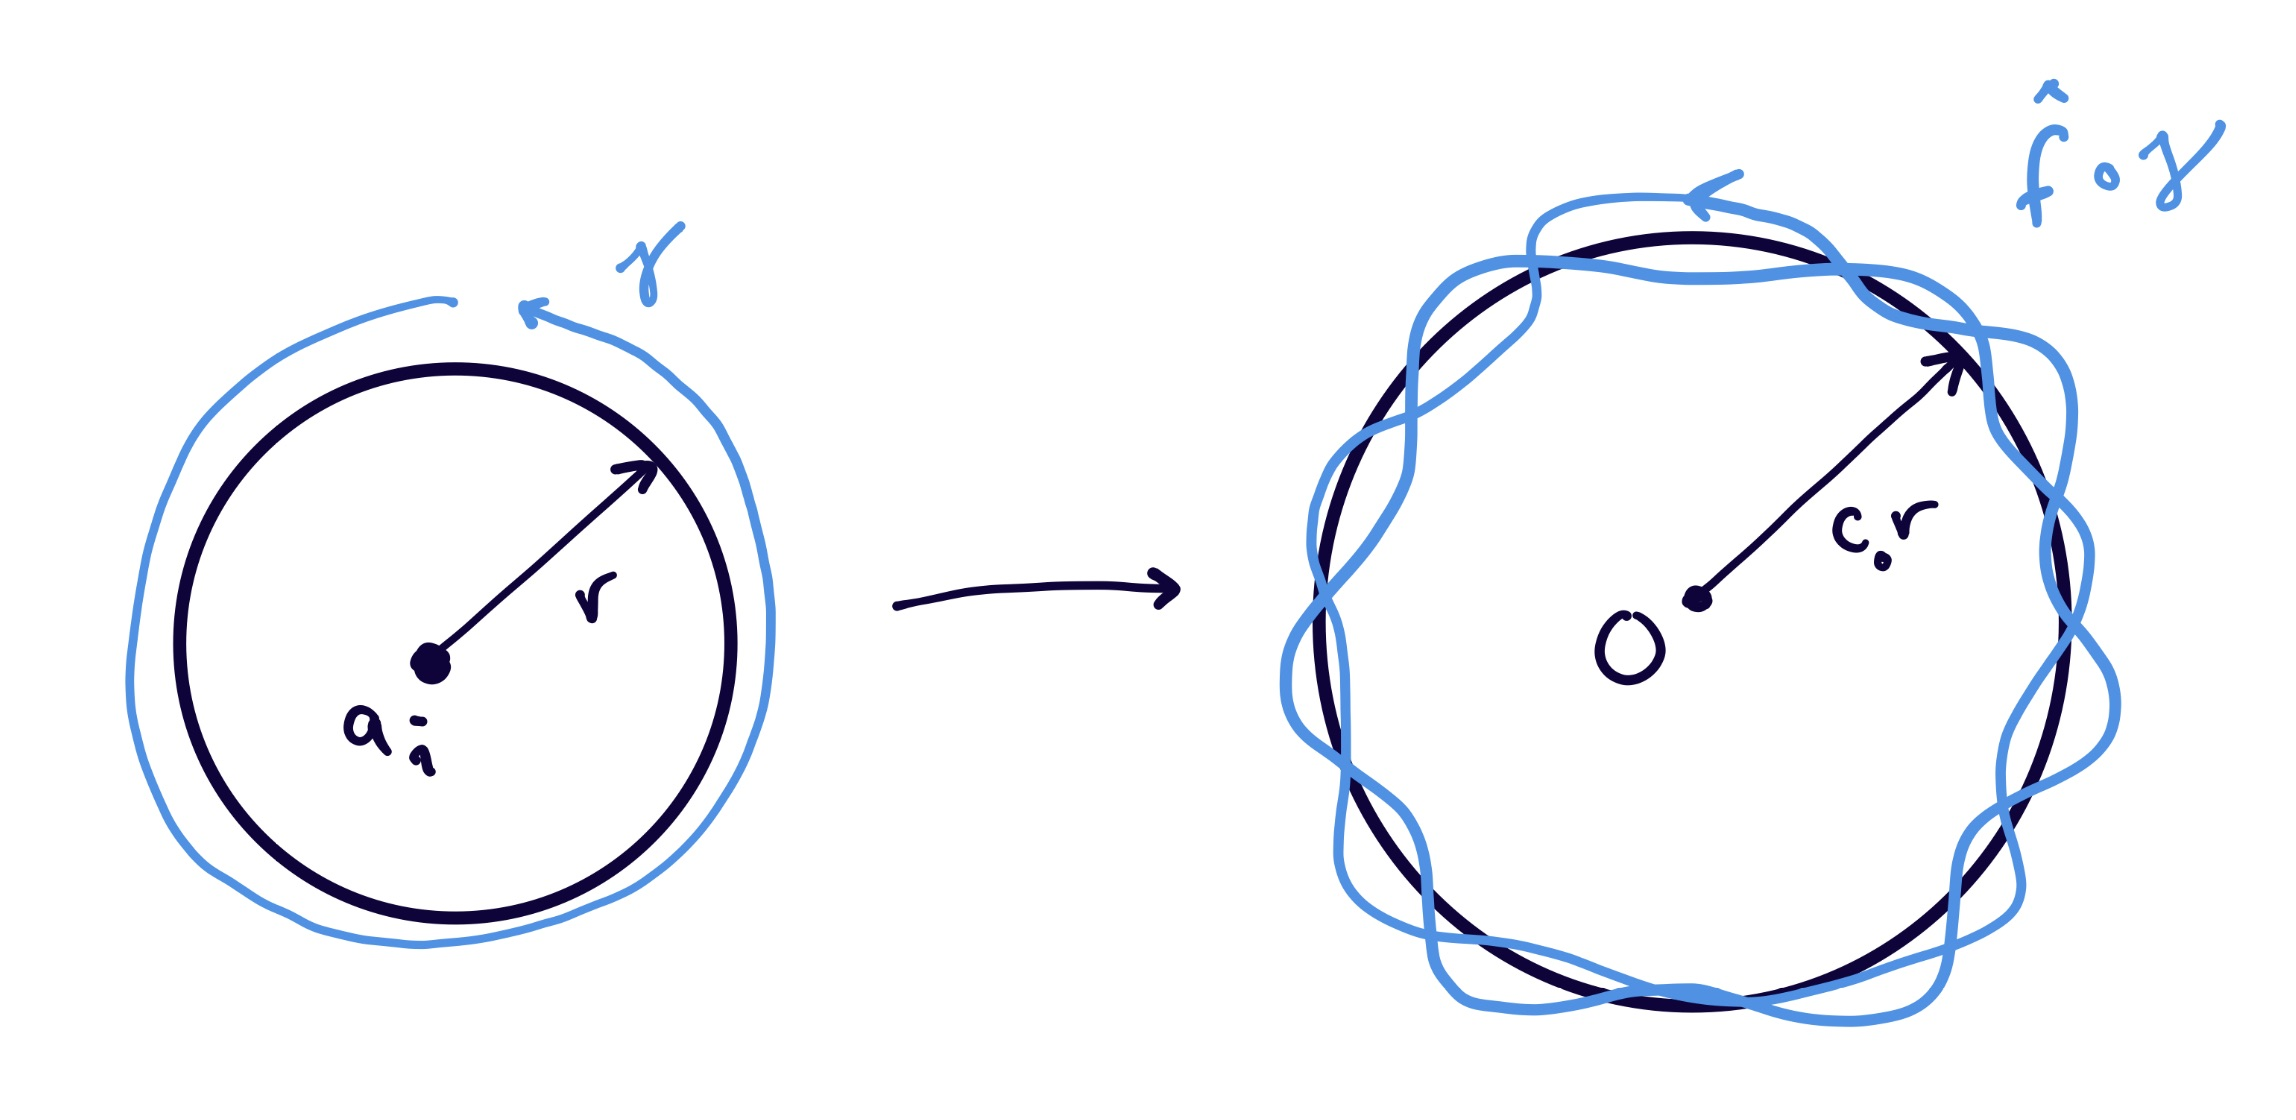
\includegraphics[width=12cm]{figures/hwk10-fig1.png}
      \captionof{figure}{The map $\hatf \circ \gamma$ is $c_0(z - a_i)^{d_i}$ plus some wobble.}
      \label{fig:prob1-1}
    \end{center}
  \end{prf} 
  \prob[\textsc{Exercise 12.}] Show that the quotient map $S^1\times S^1 \to S^2$ collapsing the subspace $S^1 \vee S^1$ to a point is not nullhomotopic by showing that it induces an isomorphism on $H_2$. On the other hand, show via covering spaces that any map $S^2 \to S^1\vee S^1$ is null homo topic.
  \begin{prf}
    We first note that $(S_1\times S^1, S^1\vee S^1)$ is a good pair. Indeed, we can take a tubular neighborhood of $S^1\vee S^1$ inside $S^1\times S^1$ which deformation retracts to $S^1\vee S^1$, as illustrated in Figure \ref{fig:prob12-2}.
    \begin{center}
      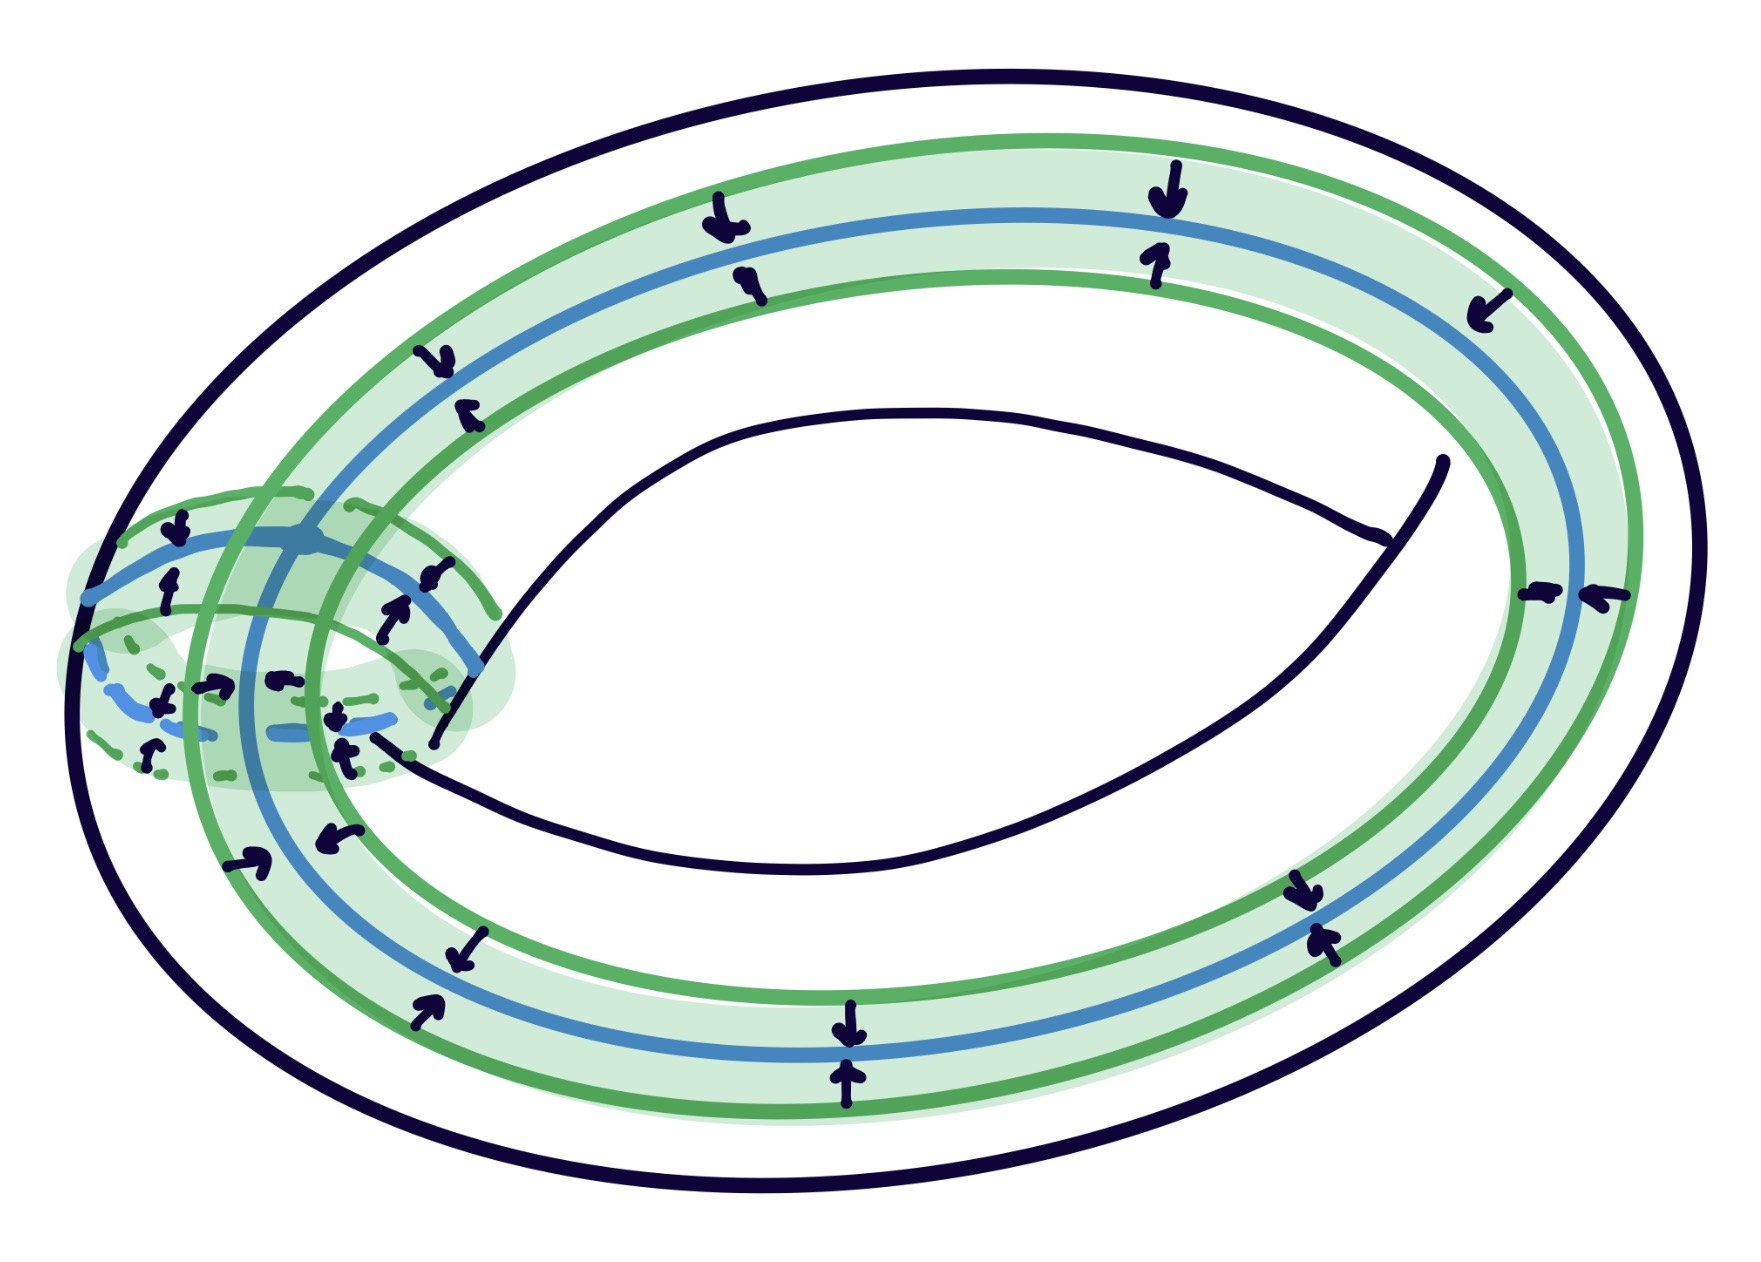
\includegraphics[width=10cm]{figures/hwk10-fig2.png}
      \captionof{figure}{Tubular neighborhood deformation retracts onto $S^1\vee S^1$.}
      \label{fig:prob12-2}
    \end{center}
    Theorem 2.13 from Hitcher then implies that we have a long exact sequence
    \begin{align*}
      ...\to H_2(S^1\vee S^1) \to H_2(S^1\times S^1) \xrightarrow{p_*} H_2(S^2) \xrightarrow{\partial} H_1(S^1\vee S^1)\to H_2(S^1\times S^1) \xrightarrow{p_*} ...
    \end{align*}
    where $p:S^1\times S^1\to S^1\times S^1/S^1\vee S^1 \cong S^2$ is the quotient map in question. As is standard practice by now, let's fill in this sequence with friendlier looking symbols for our groups and consider the relevant maps more closely:
    \begin{align*}
      ...\to 0 \to \bZ \xrightarrow{p_*} \bZ \xrightarrow{\partial} \bZ^2 \xrightarrow{i} \bZ^2 \xrightarrow{p_*},
    \end{align*}
    where $i$ is the map induced by the inclusion $S^1\vee S^1 \hookrightarrow S^1 \times S^1$. This is a cellular map which takes the two 1-cells of $S^1\vee S^1$ to 1-cells in $S^1\times S^1$; hence it is injective. This implies that $\img \partial = \ker i = 0$, and thus that $\img p_* = \ker \partial = \bZ$. Since exactness on the left side of $p_*$ implies that $p_*$ is injective, we conclude that it is an isomorphism and hence that $p$ is not nullhomotopic.

    Now let $p:\bR^2 \to S^1\times S^1$ be the universal cover of $S^1\times S^1$. Any map $f:S^2\to S^1\times S^1$ satisfies $f_*(\pi_1(S^2,s_0)) = p_*(\pi_1(\bR^2,x_0))$ since both $\pi_1(S^2,s_0)$ and $\pi_1(\bR^2,x_0)$ are trivial (here we implicitly assume $f(s_0) = p(x_0)$, as basepoints need to be compatible). By the covering space lifting property (I remember the theorem but am not sure about the name) we have a lift $g:S^2 \to \bR^2$ of $f$, but $g$ is nullhomotopic since $\bR^2$ is contractible, so $f$ must be as well.
  \end{prf}
\end{homework}
\tchap{Problems from 2.B}
\begin{homework}[e]
  \prob[\textsc{Exercise 1.}] Compute $H_i(S^n - X)$ when $X$ is a subspace of $S^n$ homeomorphic to $S^k\vee S^\ell$ or to $S^k \sqcup S^\ell$.
  \begin{prf}
    Suppose first that $X \cong S^k \sqcup S^\ell$. Denote the two connected components of $X$ inside $S^n$ by $X_1 \cong S^k$ and $X_2 \cong S^\ell$. I hope that I can use the results in section 2B of Hatcher, for proposition 2B.1.b conveniently tells us that
    \begin{align*}
      \tilH_i(S^n - X_1) \cong
      \begin{cases}
        \bZ & i = n - k - 1 \\
        0 & \text{else}
      \end{cases}, \hspace{1em}
      \tilH_i(S^n - X_2) \cong
      \begin{cases}
        \bZ & i = n - \ell - 1 \\
        0 & \text{else}
      \end{cases}.
    \end{align*}
    Let $A$ be an open set which deformation retracts to $S^n - X_1$ and similarly $B$ an open set which deformation retracts to $X_2$; this can be done by the standard process of ``thickening'' $X_1$ and $X_2$, i.e. by choosing an appropriate tubular neighborhood. We then get that $A \cup B = S^n$ while $A\cap B$ deformation retracts to $X_1\cup X^2$. This allows us to apply Mayer-Vietoris:
    \begin{align*}
      ...\to \tilH_{i+1}(S^n)\to \tilH_i(S^n - X) \to \tilH_i(S^n - X_1) \oplus \tilH_i(S^n - X_2) \to \tilH_i(S^n) \to ...
    \end{align*}
    We have three obvious indices to look at, $i = n,\ell $ and $k$. Because $k,\ell < n$, we get that $\tilH_i(S^n - X_1) = \tilH_i(S^n - X_2) = 0$ by Proposition 2B.1.b, so this section of Mayer-Vietoris reads
    \begin{align*}
      ... \to 0 \to \tilH_n(S^n - X) \to 0 \to \bZ \to ...
    \end{align*}
    and hence $\tilH_n(S^n - X)\cong 0$. This same argument holds for all $i > n$ too.

    Suppose now that both $k$ and $\ell$ are nonzero. Then
    \begin{align*}
      ... \to 0 \to \tilH_i(S^n - X) \to \tilH_i(S^n - X_1) \oplus \tilH_i(S^n - X_2) \to 0 \to ...
    \end{align*}
    is the relevant section of the Mayer-Vietoris sequence $i < n - 1$. The portions to consider are the cases when $i = n - k - 1$ and $i = n - \ell - 1$ as these yield $\bZ$'s in the sequence (in the case that either $k$ or $\ell$ are $0$, then we need to investigate $i = n - 1$, which becomes complicated). In any case, when $i = n - \ell - 1$ or $i = n - k - 1$, we have
    \begin{align*}
      0 \to \tilH_i(S^n - X) \to \tilH_i(S^n - X_1) \oplus \tilH_i(S^n - X_2) \to 0
    \end{align*}
    which means $\tilH_i(S^n - X)$ is $\bZ$ if $k \neq \ell$ and $\bZ^2$ if $k = \ell$
    At all other positions except at $i = 0$ and $i = n-1$ we have only trivial terms in the sequence. When $i = n-1$ we have
    \begin{align*}
      ... \to 0 \to \bZ \to \tilH_{n-1}(S^n - X) \to 0 \to ...
    \end{align*}
    which yields an isomorphism $\tilH_{n-1}(S^n - X) \cong \bZ$. At $i = 0$ we get
    \begin{align*}
      0 \to \tilH_0(S^n - X) \to \tilH_0(S^n - X_1) \oplus \tilH_0(S^n - X_2) \to 0
    \end{align*}
    which implies $\tilH_0(S^n - X) = 0\implies H_0(S^n - X)\cong \bZ$. To summarize, when $k,\ell \neq 0$,
    \begin{align*}
      H_i(S^n - X) \cong
      \begin{cases}
        \bZ & i = 0 \\
        \bZ & i \in \{n- k - 1, n - \ell - 1, n-1\} \text{ and } k\neq \ell\\
        \bZ^2 & i = n - k - 1 \text{ and } k = \ell \\
        0 & \text{otherwise}
      \end{cases}.
    \end{align*}
    There are a few extraneous cases that fit into the $k, \ell \neq 0$ situation that we have not considered. For instance, if either $k = n - 1$ or $\ell = n-1$ a similar thing occurs as in the $k = \ell$ case occurs; we get $H_i(S^n - X) = \bZ^2$ in the $i = 0$. Additionally, if $n = 1$, then $k = \ell = n - 1 = 0$. This means $S^n - X$ is really the removal of two copies of $S^0$ from $S^1$, which results in four path components and hence $H_0(S^1 - X) \cong \bZ^4$.

    \bigskip

    Now suppose that $k \neq 0$ and $\ell = 0$. Our homology remains unchanged except in the case that $i = n-\ell - 1 = n - 1$, where the Mayer-Vietoris sequence becomes
    \begin{align*}
      ...\to 0 \to \bZ \to \tilH_{n-1}(S^n - X) \to \bZ \to 0 \to ...
    \end{align*}
    where we note that $\tilH_{n-1}(S^n - X^k) \cong 0$ since $k \neq 0$. Because $\bZ$ is free, this sequence splits and we get that $\tilH_i(S^n - X) \cong \bZ \oplus \bZ$. All other homology groups remain unchanged from before.

    \bigskip

    Finally, if both $\ell = k = 0$ then we get
    \begin{align*}
      ...\to 0 \to \bZ \to \tilH_{n-1}(S^n - X) \to \bZ \oplus \bZ\to 0 \to ...
    \end{align*}
    when $i = n-1$. This also splits because $\bZ\oplus \bZ$ is still free, so $\tilH_{n-1}(S^n - X) = \bZ\oplus \bZ\oplus \bZ$. To summarize all these cases in a succinct way:
    \begin{align*}
      H_i(S^n - X) \cong
      \begin{cases}
        \bZ & i = 0, n-k - 1, n - \ell - 1, n-1 \\
        0 & \text{otherwise}
      \end{cases}
    \end{align*}
    and we merge the $\bZ$'s together with direct sums if any of the $0,n - \ell - 1, n - k - 1, n - 1$ terms coincide.

    \bigskip

    Now recall that this is only half of the problem -- we still need to treat the $X \cong S^k \vee S^\ell$ case. Luckily, there are not as many cases to think about here. Once again, denote by $X_1$ the copy of $S^k$ in $X$ and by $X_2$ the copy of $S^{\ell}$ in $X$. We still have that
    \begin{align*}
      \tilH_i(S^n - X_1) \cong
      \begin{cases}
        \bZ & i = n - k - 1 \\
        0 & \text{else}
      \end{cases}, \hspace{1em}
      \tilH_i(S^n - X_2) \cong
      \begin{cases}
        \bZ & i = n - \ell - 1 \\
        0 & \text{else}
      \end{cases}.
    \end{align*}
    by Proposition 2B.1.b. Using the same $A$ and $B$ as before, we get $A\cup B = S^n - \{p\}$ where $p$ is the point at which $X_1$ and $X_2$ meet. It's still true that $A \cap B$ deformation retracts to $X$. The removal of one point from $S^n$ results in $\bR^n$, which is contractible, so $A \cup B \simeq \{pt\}$. Mayer-Vietoris therefore gives
    \begin{align*}
      ... \to 0 \to \tilH_i(S^n - X) \to \tilH_i(S^n - X_1) \oplus \tilH_i(X^n - X_2) \to 0 \to ...
    \end{align*}
    for \emph{all} $i$ (yay!), and we get $\tilH_i(S^n - X) \cong \tilH_i(S^n - X_1) \oplus \tilH_i(X^n - X_2) \cong \bZ \oplus \bZ$. In summary,
    \begin{align*}
      H_i(S^n - X) \cong
      \begin{cases}
        \bZ & i = 0, n - k - 1, n - \ell - 1 \\
        0 & \text{else}
      \end{cases}.
    \end{align*}
  \end{prf}
  \prob[\textsc{Exercise 2.}] Show that $\tilH_i(S^n - X) \cong \tilH_{n - i - 1}(X)$ when $X$ is homeomorphic to a finite connected graph. [First do the case that $X$ is a tree.]
  \begin{prf}
    Starting with a tree is nice because trees are always contractible. This means in particular $\tilH_{n - i - 1}(X) \cong 0$. Intuitively, deleting a tree from the surface of $S^n$ gives us a space homeomorphic to $\bR^n$, which is also contractible. This nonetheless demands more justification, so we proceed inductively on the number of vertices contained in $X$, a number which we denote by $V_X$. 

    When $V_X = 1$, $S^n - X$ truly is just the one-point-uncompactification of $S^n$ and is thus contractible, so our base case is clear. Now suppose that $\tilH_i(S^n - X) = 0$ when $V_X \leq k$. Consider the case then that $V_X = k+1$. Since $X$ is a tree, there is some vertex $v$ with only one edge attached. Call this one edge $e$ and the other vertex to which it connects $w$. Consider the deformation retract of $X$ which collapses $e$; this produces a new tree $Y$ with only $k$ vertices. Set $A = S^n - e$ and $B = S^n - Y$, noting that these are both open sets. Then $A \cup B = S^n - \{v\}$ and $A\cap B = S^n - X$, so we are in a good position to apply Mayer-Vietoris:
    \begin{align*}
      ... \to \tilH_{i+1}(S^n - \{v\}) \to \tilH_i(S^n - X) \to \tilH_i(S^n - e) \oplus \tilH_i(S^n - Y) \to \tilH_i(S^n - \{v\}) \to ...
    \end{align*}
    Applying the inductive hypothesis gives us
    \begin{align*}
      ... \to 0 \to \tilH_i(S^n - X) \to 0 \to 0 \to ...
    \end{align*}
    and so $\tilH_i(S^n\setminus X)\cong 0$, as desired. Notice that we haven't proven that $S^n - X$ is contractible, only that it has trivial homology.

    \bigskip

    Now let $X$ be homeomorphic to some finite graph. Denote by $T$ the maximal subtree of $X$. If $T = X$ then we are done by what we have already shown; assume then that $T \subsetneq X$. We'll proceed by induction on the number of edges of $X \setminus T$. Think of the size of this set as indicating ``how far $X$ is from being a tree.'' Our base case is out of the way already by the $X\setminus T = \emptyset$ case, so assume that $\tilH_i(S^n - X) \cong \tilH_{n-i-1}(X)$ whenever $|E(X\setminus T)| \leq k$ and that we have $|E(X\setminus T)| = k + 1$. Write $X = X' \cup e$, where $e$ is one of the edges not in $T$ and $X'$ is a graph with $k$ edges not in $T$. It follows from the inductive hypothesis that $\tilH_i(S^n - X') \cong \tilH_{n-i-1}(X')$. This second group is actually computable; since $X'$ has $k$ edges not in the maximal subtree, after collapsing $T$ to a point we obtain a wedge of $k$ circles. Hence
    \begin{align*}
      \tilH_{i}(X') \cong
      \begin{cases}
        \bZ^m & i = 1 \\
        0 & else
      \end{cases}.
    \end{align*}
    Because $X$ is a simple graph, it has no loops formed by an edge connecting twice to a single vertex. This implies that $X' \cap e$ consists of precisely two points $v$ and $u$. Both of these points are in $T$ since maximal subtrees contain every vertex and in $X'$ since $T \subseteq X'$. We now apply Mayer-Vietoris using open sets $A = S^n - e$ and $B = S^n - Y$. We have $A\cup B = S^n - \{v,u\} \cong S^{n-1}$ and $A\cap B = S^n \setminus X$. MV yields
    \begin{align*}
      ... \to \tilH_{i+1}(S^{n-1}) \to \tilH_i(S^n - X) \to \tilH_i(S^n - e) \oplus \tilH_i(S^n - Y) \to \tilH_i(S^{n-1})\to ...
    \end{align*}
    If $i \neq n-1$ or $n-2$, then we get
    \begin{align*}
      ...\to 0 \to \tilH_i(S^n \setminus X) \to \tilH_i(S^n - X') \to 0 \to ...
    \end{align*}
    which gives us an isomorphism $\tilH_i(S^n - X)\cong \tilH_i(S^n- X')$. Because $\tilH_i(S^n - X') = 0$ unless $i = n-2$, a case that we are not in, $\tilH_i(S^n - X) = 0$ for all $i \neq n - 1, n - 2$.

    Now consider $i = n - 1$. The relevant portion of MV is
    \begin{align*}
      ...\to 0 \to \tilH_i(S^n \setminus X) \to \tilH_i(S^n - X') \to \bZ \to ...
    \end{align*}
    but since $\tilH_n(S^n - X') \cong 0$, we get $\tilH_{n-1}(S^n - X) = 0$ too. All that remains is the $i = n-2$ case:
    \begin{align*}
      ... \to 0 \to \tilH_{n-1}(S^{n-1}) \to \tilH_{n-2}(S^{n} - X) \to \tilH_{n - 2}(S^n - Y) \to 0 ...
    \end{align*}
    where we have used the facts that $\tilH_{n-1}(S^{n-1}) = \tilH_{n-2}(S^{n-1}) = 0$. The two outer groups are both free, so we have a short exact sequence which splits:
    \begin{align*}
      ... \to 0 \to \bZ \to \tilH_{n-2}(S^n - X) \to \bZ^m \to 0 \to ...
    \end{align*}
    and so $\tilH_{n-2}(S^n - X) = \bZ^{m+1}$ when $i = n - 2$ and is 0 everywhere else. This is identical to $\tilH_{n - i - 1}(X)$, which we can compute in the same way as $X'$ by collapsing $T$ to a point and realizing we've obtained a wedge of $m + 1$ circles.
  \end{prf}
\end{homework}
\end{document}
